\documentclass{standalone}
\usepackage{tikz}
\usetikzlibrary{patterns, positioning}


\begin{document}
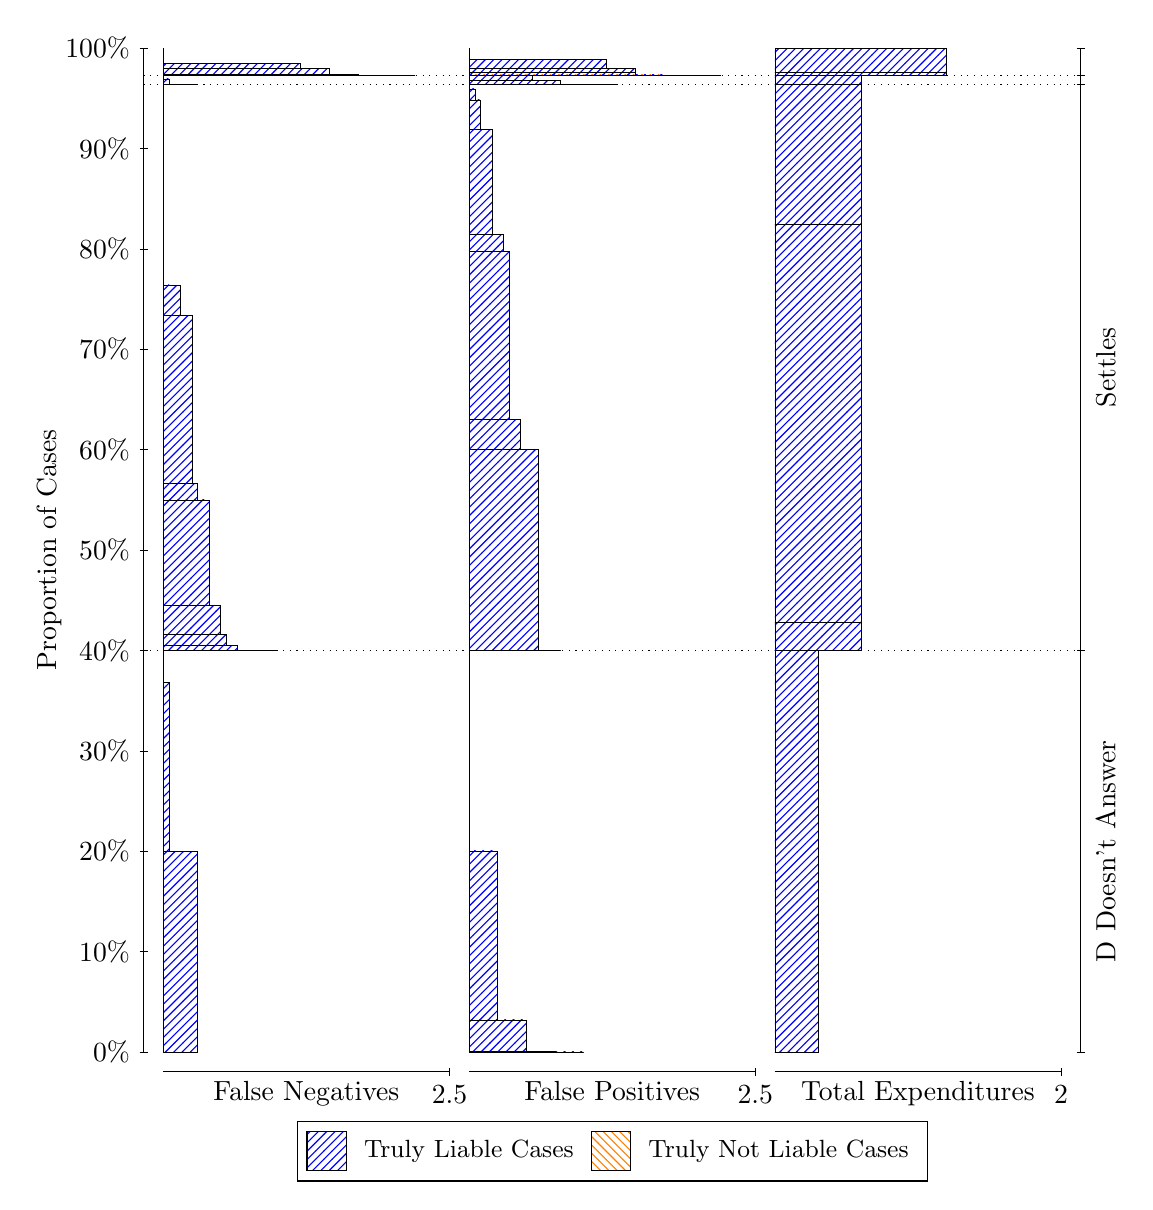
\begin{tikzpicture}
\draw[black, very thin] (1.5,1.75) -- (1.5,14.5);
\node[rotate=90, text=black, anchor=center] at (0.3, 8.125) {Proportion of Cases};
\draw[black, very thin] (1.45,1.75) -- (1.55,1.75);
\node[text=black, anchor=east] at (1.45, 1.75) {0\%};
\draw[black, very thin] (1.45,3.025) -- (1.55,3.025);
\node[text=black, anchor=east] at (1.45, 3.025) {10\%};
\draw[black, very thin] (1.45,4.3) -- (1.55,4.3);
\node[text=black, anchor=east] at (1.45, 4.3) {20\%};
\draw[black, very thin] (1.45,5.575) -- (1.55,5.575);
\node[text=black, anchor=east] at (1.45, 5.575) {30\%};
\draw[black, very thin] (1.45,6.85) -- (1.55,6.85);
\node[text=black, anchor=east] at (1.45, 6.85) {40\%};
\draw[black, very thin] (1.45,8.125) -- (1.55,8.125);
\node[text=black, anchor=east] at (1.45, 8.125) {50\%};
\draw[black, very thin] (1.45,9.4) -- (1.55,9.4);
\node[text=black, anchor=east] at (1.45, 9.4) {60\%};
\draw[black, very thin] (1.45,10.675) -- (1.55,10.675);
\node[text=black, anchor=east] at (1.45, 10.675) {70\%};
\draw[black, very thin] (1.45,11.95) -- (1.55,11.95);
\node[text=black, anchor=east] at (1.45, 11.95) {80\%};
\draw[black, very thin] (1.45,13.225) -- (1.55,13.225);
\node[text=black, anchor=east] at (1.45, 13.225) {90\%};
\draw[black, very thin] (1.45,14.5) -- (1.55,14.5);
\node[text=black, anchor=east] at (1.45, 14.5) {100\%};

\draw[black, very thin] (13.4,1.75) -- (13.4,14.5);
\draw[black, very thin] (13.35,1.75) -- (13.45,1.75);
\node[anchor=west] at (13.35, 1.75) {};
\draw[black, very thin] (13.35,6.8488) -- (13.45,6.8488);
\node[anchor=west] at (13.35, 6.8488) {};
\draw[black, very thin] (13.35,14.042) -- (13.45,14.042);
\node[anchor=west] at (13.35, 14.042) {};
\draw[black, very thin] (13.35,14.155) -- (13.45,14.155);
\node[anchor=west] at (13.35, 14.155) {};
\draw[black, very thin] (13.35,14.5) -- (13.45,14.5);
\node[anchor=west] at (13.35, 14.5) {};

\draw[black, very thin, pattern color=blue, pattern=north east lines] (1.75,1.75) rectangle (2.186,4.2958);
\draw[black, very thin, pattern color=blue, pattern=north east lines] (1.75,4.2958) rectangle (1.8227,6.4407);
\draw[black, very thin, pattern color=orange, pattern=north west lines] (1.75,6.4407) rectangle (1.75,6.4407);
\draw[black, very thin, pattern color=blue, pattern=north east lines] (1.75,6.4407) rectangle (1.75,6.8488);
\draw[black, very thin, pattern color=blue, pattern=north east lines] (1.75,6.8488) rectangle (3.2033,6.8488);
\draw[black, very thin, pattern color=blue, pattern=north east lines] (1.75,6.8488) rectangle (3.058,6.8488);
\draw[black, very thin, pattern color=blue, pattern=north east lines] (1.75,6.8488) rectangle (2.9127,6.8492);
\draw[black, very thin, pattern color=blue, pattern=north east lines] (1.75,6.8492) rectangle (2.84,6.852);
\draw[black, very thin, pattern color=blue, pattern=north east lines] (1.75,6.852) rectangle (2.6947,6.9094);
\draw[black, very thin, pattern color=blue, pattern=north east lines] (1.75,6.9094) rectangle (2.5493,7.0502);
\draw[black, very thin, pattern color=blue, pattern=north east lines] (1.75,7.0502) rectangle (2.4767,7.426);
\draw[black, very thin, pattern color=blue, pattern=north east lines] (1.75,7.426) rectangle (2.3313,8.7608);
\draw[black, very thin, pattern color=blue, pattern=north east lines] (1.75,8.7608) rectangle (2.186,8.9711);
\draw[black, very thin, pattern color=blue, pattern=north east lines] (1.75,8.9711) rectangle (2.1133,11.107);
\draw[black, very thin, pattern color=blue, pattern=north east lines] (1.75,11.107) rectangle (1.968,11.488);
\draw[black, very thin, pattern color=blue, pattern=north east lines] (1.75,11.488) rectangle (1.8227,11.493);
\draw[black, very thin, pattern color=orange, pattern=north west lines] (1.75,11.493) rectangle (1.75,11.493);
\draw[black, very thin, pattern color=blue, pattern=north east lines] (1.75,11.493) rectangle (1.75,14.042);
\draw[black, very thin, pattern color=blue, pattern=north east lines] (1.75,14.042) rectangle (2.186,14.043);
\draw[black, very thin, pattern color=blue, pattern=north east lines] (1.75,14.043) rectangle (1.8227,14.107);
\draw[black, very thin, pattern color=orange, pattern=north west lines] (1.75,14.107) rectangle (1.75,14.107);
\draw[black, very thin, pattern color=blue, pattern=north east lines] (1.75,14.107) rectangle (1.75,14.155);
\draw[black, very thin, pattern color=blue, pattern=north east lines] (1.75,14.155) rectangle (4.9473,14.155);
\draw[black, very thin, pattern color=blue, pattern=north east lines] (1.75,14.155) rectangle (4.584,14.156);
\draw[black, very thin, pattern color=blue, pattern=north east lines] (1.75,14.156) rectangle (4.2207,14.163);
\draw[black, very thin, pattern color=blue, pattern=north east lines] (1.75,14.163) rectangle (3.8573,14.241);
\draw[black, very thin, pattern color=blue, pattern=north east lines] (1.75,14.241) rectangle (3.494,14.301);
\draw[black, very thin, pattern color=blue, pattern=north east lines] (1.75,14.301) rectangle (3.1307,14.301);
\draw[black, very thin, pattern color=blue, pattern=north east lines] (1.75,14.301) rectangle (2.7673,14.301);
\draw[black, very thin, pattern color=blue, pattern=north east lines] (1.75,14.301) rectangle (2.4767,14.301);
\draw[black, very thin, pattern color=blue, pattern=north east lines] (1.75,14.301) rectangle (2.1133,14.303);
\draw[black, very thin, pattern color=orange, pattern=north west lines] (1.75,14.303) rectangle (1.75,14.303);
\draw[black, very thin, pattern color=blue, pattern=north east lines] (1.75,14.303) rectangle (1.75,14.5);
\draw[black, very thin, pattern color=orange, pattern=north west lines] (5.6333,1.75) rectangle (7.0867,1.75);
\draw[black, very thin, pattern color=blue, pattern=north east lines] (5.6333,1.75) rectangle (7.0867,1.75);
\draw[black, very thin, pattern color=blue, pattern=north east lines] (5.6333,1.75) rectangle (6.7233,1.7535);
\draw[black, very thin, pattern color=blue, pattern=north east lines] (5.6333,1.7535) rectangle (6.36,2.158);
\draw[black, very thin, pattern color=blue, pattern=north east lines] (5.6333,2.158) rectangle (5.9967,4.303);
\draw[black, very thin, pattern color=blue, pattern=north east lines] (5.6333,4.303) rectangle (5.6333,6.8488);
\draw[black, very thin, pattern color=orange, pattern=north west lines] (5.6333,6.8488) rectangle (6.796,6.8488);
\draw[black, very thin, pattern color=blue, pattern=north east lines] (5.6333,6.8488) rectangle (6.796,6.8488);
\draw[black, very thin, pattern color=orange, pattern=north west lines] (5.6333,6.8488) rectangle (6.6507,6.8488);
\draw[black, very thin, pattern color=blue, pattern=north east lines] (5.6333,6.8488) rectangle (6.6507,6.8527);
\draw[black, very thin, pattern color=orange, pattern=north west lines] (5.6333,6.8527) rectangle (6.5053,6.8527);
\draw[black, very thin, pattern color=blue, pattern=north east lines] (5.6333,6.8527) rectangle (6.5053,9.3985);
\draw[black, very thin, pattern color=blue, pattern=north east lines] (5.6333,9.3985) rectangle (6.4327,9.4027);
\draw[black, very thin, pattern color=blue, pattern=north east lines] (5.6333,9.4027) rectangle (6.2873,9.7845);
\draw[black, very thin, pattern color=blue, pattern=north east lines] (5.6333,9.7845) rectangle (6.142,11.92);
\draw[black, very thin, pattern color=blue, pattern=north east lines] (5.6333,11.92) rectangle (6.0693,12.13);
\draw[black, very thin, pattern color=blue, pattern=north east lines] (5.6333,12.13) rectangle (5.924,13.465);
\draw[black, very thin, pattern color=blue, pattern=north east lines] (5.6333,13.465) rectangle (5.7787,13.841);
\draw[black, very thin, pattern color=blue, pattern=north east lines] (5.6333,13.841) rectangle (5.706,13.982);
\draw[black, very thin, pattern color=blue, pattern=north east lines] (5.6333,13.982) rectangle (5.6333,14.042);
\draw[black, very thin, pattern color=orange, pattern=north west lines] (5.6333,14.042) rectangle (7.5227,14.042);
\draw[black, very thin, pattern color=blue, pattern=north east lines] (5.6333,14.042) rectangle (7.5227,14.042);
\draw[black, very thin, pattern color=blue, pattern=north east lines] (5.6333,14.042) rectangle (7.1593,14.043);
\draw[black, very thin, pattern color=blue, pattern=north east lines] (5.6333,14.043) rectangle (6.796,14.091);
\draw[black, very thin, pattern color=blue, pattern=north east lines] (5.6333,14.091) rectangle (6.4327,14.154);
\draw[black, very thin, pattern color=blue, pattern=north east lines] (5.6333,14.154) rectangle (6.0693,14.155);
\draw[black, very thin, pattern color=orange, pattern=north west lines] (5.6333,14.155) rectangle (8.8307,14.155);
\draw[black, very thin, pattern color=blue, pattern=north east lines] (5.6333,14.155) rectangle (8.8307,14.155);
\draw[black, very thin, pattern color=blue, pattern=north east lines] (5.6333,14.155) rectangle (8.4673,14.155);
\draw[black, very thin, pattern color=orange, pattern=north west lines] (5.6333,14.155) rectangle (8.4673,14.155);
\draw[black, very thin, pattern color=blue, pattern=north east lines] (5.6333,14.155) rectangle (8.4673,14.155);
\draw[black, very thin, pattern color=blue, pattern=north east lines] (5.6333,14.155) rectangle (8.104,14.159);
\draw[black, very thin, pattern color=orange, pattern=north west lines] (5.6333,14.159) rectangle (8.104,14.159);
\draw[black, very thin, pattern color=blue, pattern=north east lines] (5.6333,14.159) rectangle (8.104,14.16);
\draw[black, very thin, pattern color=blue, pattern=north east lines] (5.6333,14.16) rectangle (7.7407,14.193);
\draw[black, very thin, pattern color=blue, pattern=north east lines] (5.6333,14.193) rectangle (7.7407,14.239);
\draw[black, very thin, pattern color=blue, pattern=north east lines] (5.6333,14.239) rectangle (7.3773,14.241);
\draw[black, very thin, pattern color=blue, pattern=north east lines] (5.6333,14.241) rectangle (7.3773,14.353);
\draw[black, very thin, pattern color=blue, pattern=north east lines] (5.6333,14.353) rectangle (7.014,14.354);
\draw[black, very thin, pattern color=blue, pattern=north east lines] (5.6333,14.354) rectangle (6.6507,14.354);
\draw[black, very thin, pattern color=orange, pattern=north west lines] (5.6333,14.354) rectangle (6.36,14.354);
\draw[black, very thin, pattern color=blue, pattern=north east lines] (5.6333,14.354) rectangle (6.36,14.354);
\draw[black, very thin, pattern color=orange, pattern=north west lines] (5.6333,14.354) rectangle (5.9967,14.354);
\draw[black, very thin, pattern color=blue, pattern=north east lines] (5.6333,14.354) rectangle (5.9967,14.354);
\draw[black, very thin, pattern color=orange, pattern=north west lines] (5.6333,14.354) rectangle (5.6333,14.354);
\draw[black, very thin, pattern color=blue, pattern=north east lines] (5.6333,14.354) rectangle (5.6333,14.5);
\draw[black, very thin, pattern color=orange, pattern=north west lines] (9.5167,1.75) rectangle (10.062,1.75);
\draw[black, very thin, pattern color=blue, pattern=north east lines] (9.5167,1.75) rectangle (10.062,6.8488);
\draw[black, very thin, pattern color=orange, pattern=north west lines] (9.5167,6.8488) rectangle (10.607,6.8488);
\draw[black, very thin, pattern color=blue, pattern=north east lines] (9.5167,6.8488) rectangle (10.607,7.2044);
\draw[black, very thin, pattern color=orange, pattern=north west lines] (9.5167,7.2044) rectangle (10.607,7.2044);
\draw[black, very thin, pattern color=blue, pattern=north east lines] (9.5167,7.2044) rectangle (10.607,12.264);
\draw[black, very thin, pattern color=orange, pattern=north west lines] (9.5167,12.264) rectangle (10.607,12.264);
\draw[black, very thin, pattern color=blue, pattern=north east lines] (9.5167,12.264) rectangle (10.607,14.042);
\draw[black, very thin, pattern color=orange, pattern=north west lines] (9.5167,14.042) rectangle (10.607,14.042);
\draw[black, very thin, pattern color=blue, pattern=north east lines] (9.5167,14.042) rectangle (10.607,14.155);
\draw[black, very thin, pattern color=orange, pattern=north west lines] (9.5167,14.155) rectangle (11.697,14.155);
\draw[black, very thin, pattern color=blue, pattern=north east lines] (9.5167,14.155) rectangle (11.697,14.194);
\draw[black, very thin, pattern color=orange, pattern=north west lines] (9.5167,14.194) rectangle (11.697,14.194);
\draw[black, very thin, pattern color=blue, pattern=north east lines] (9.5167,14.194) rectangle (11.697,14.5);
\draw[black, dotted] (1.5,6.8488) -- (13.4,6.8488);
\draw[black, dotted] (1.5,14.042) -- (13.4,14.042);
\draw[black, dotted] (1.5,14.155) -- (13.4,14.155);
\draw[black, very thin] (1.75,1.5) -- (5.3833,1.5);
\node[text=black, anchor=north] at (3.5667, 1.5) {False Negatives};
\draw[black, very thin] (5.3833,1.45) -- (5.3833,1.55);
\node[text=black, anchor=north] at (5.3833, 1.45) {2.5};

\draw[black, very thin] (5.6333,1.5) -- (9.2667,1.5);
\node[text=black, anchor=north] at (7.45, 1.5) {False Positives};
\draw[black, very thin] (9.2667,1.45) -- (9.2667,1.55);
\node[text=black, anchor=north] at (9.2667, 1.45) {2.5};

\draw[black, very thin] (9.5167,1.5) -- (13.15,1.5);
\node[text=black, anchor=north] at (11.333, 1.5) {Total Expenditures};
\draw[black, very thin] (13.15,1.45) -- (13.15,1.55);
\node[text=black, anchor=north] at (13.15, 1.45) {2};

\node[text=black, centered, rotate=90] at (13.72, 4.2994) {D Doesn't Answer};
\node[text=black, centered, rotate=90] at (13.72, 10.446) {Settles};



\draw (7.449999999999999,1.5) node[draw=none] (baseCoordinate) {};
\begin{scope}[align=center]
        \matrix[scale=0.5, draw=black, below=0.5cm of baseCoordinate, nodes={draw}, column sep=0.1cm]{
            \node[rectangle, draw, minimum width=0.5cm, minimum height=0.5cm, pattern color=blue, pattern=north east lines] {}; &
            \node[draw=none, font=\small, text=black] (B) {Truly Liable Cases}; &
            \node[rectangle, draw, minimum width=0.5cm, minimum height=0.5cm, pattern color=orange, pattern=north west lines] {}; &
            \node[draw=none, font=\small, text=black] (B) {Truly Not Liable Cases}; \\
            };
\end{scope}

\end{tikzpicture}
\end{document}